\documentclass[11pt, a4paper]{article}
\usepackage{noweb}
\usepackage{amsmath}
\usepackage{a4wide}  % Set margins automatically for wider use of A4
\usepackage{graphicx}
\usepackage{float}      % place multiple floats in one float
\usepackage{subfig}     % place multiple figs in one figure
\usepackage{placeins}   % to stop floats from floating
\usepackage{wrapfig}
\noweboptions{}
\title{EE705 Course Project -- LDPC Decoder}
\author{Anuja Singh (184074001), Niraj N Sharma (184077001), Sandeep Mishra (184076005) \and Sonali Shukla (184070014)}
\date{Final Report: May 2, 2019}
\begin{document}
\maketitle
The project involves the design and layout of a LDPC decoder block. After
the creation of behavioural RTL using BSV and Verilog, we have chosen to use
an open-source ASIC design flow to generate the GDS2 for the design.

\section{LDPC Background}
In communication system normally the transmitter appends parity bits to
message bits in order allow the receiver to correct or detect errors. These
are called error correcting codes. There is a generator matrix which
encapsulates the implementation of the parity check equations :
\[
C = M*G
\]

Here, C is the coded message, M is the original message and G is the generator
matrix. At the receiver side we have the received message bit and the parity
check matrix, from which we decode the message.

In LDPC codes there is a property that every code digit is contained in the
same no. of equations and each equations contains the same no. of code
symbols. LDPC codes are usually represented by the tanner graph. Tanner graph
contains two set of vertices: 
\begin{enumerate}
   \item $n$ vertices for the code word bits called a bit nodes.
   \item $m$ vertices for the check equation called check node.
\end{enumerate}

\begin{figure}[hbt]
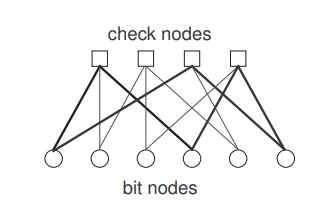
\includegraphics{pic2.png}
\label{fig:pic2}
\caption{Representation in a tanner graph}
\end{figure}

\subsection{The Parity Matrix}
The parity matrix dictates the connections between the bit-nodes and
check-nodes and encodes a tanner graph. So, in order to build a hardware LDPC
decoder, we have to fix this parity matrix. We have chosen the following
matrix which has been provided to us by Mandar J.~Datar from the HPC Lab:

\[
H = \begin{bmatrix}
1 1 0 1 0 0 0 \\
0 1 1 0 1 0 0 \\
0 0 1 1 0 1 0 \\
0 0 0 1 1 0 1 \\
1 0 0 0 1 1 0 \\
0 1 0 0 0 1 1 \\
1 0 1 0 0 0 1 \\
\end{bmatrix}
\]

A $1$ at row $i$, column $j$ indicates a connection between $i^{th}$ checknode
and $j^{th}$ bitnode as show in figure~\ref{fig:bc}.

\begin{figure}[hbt]
%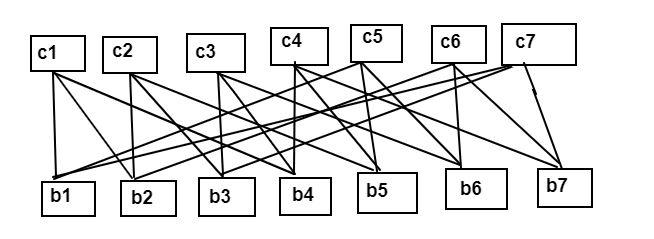
\includegraphics[width=\linewidth]{pic1.jpg}
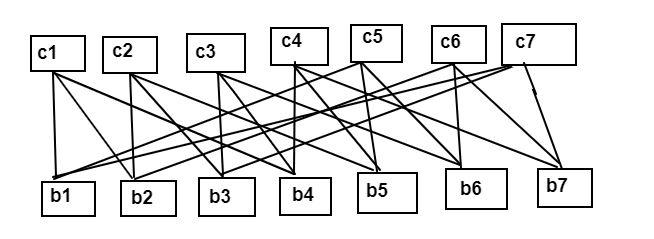
\includegraphics{pic1.jpg}
\label{fig:bc}
\caption{Bitnodes and Checknodes connections based on the given H matrix}
\end{figure}

\subsection{Decoder Algorithm}
Here we used the Bit Flipping algorithm, in which the received message bits
are decoded according to the parity matrix and if the bit obtained is not
correct, then the respective bit is flipped and then again the equations are
checked. The bit flip decoder directly gives it output whenever a valid code
word has obtained which satisfies all the parity check equation.
Here the $c_1$ means the first bit of coded word is taking the input from the
$b_1$, $b_2$, $b_4$, then bit which it will send back to the $b_0$ is:

\[
   c_1 = b_1 \oplus b_2 \oplus b_4
\]
\[
   c_2 = b_2 \oplus b_3 \oplus b_5
\]

These are sent back to the respective bitnodes. For instance bitnode-1 will
receive inputs from checknodes 1, 6 and 7 and so on. Now, the bit assigned to
the b1 is the majority of the bits which are send by the c1, c6 and c7.

Like this all the bits have one value assigned to them, now to check whether
the decoded messages bits are correct or not all the parity equations should
be checked using:
\[
   (b_1 \oplus b_2 \oplus b_4) \vee (b_2 \oplus b3 \oplus b5) \vee (b3 \oplus
   b4 \oplus b6) \vee (b4 \oplus b5 \oplus b7) \vee (b1 \oplus b5 \oplus b6)
   \vee (b2 \oplus b6 \oplus b7) \vee (b1 \oplus b3 \oplus b7)
\]
If the output of the above equation is zero means the decoded message bits are
correct otherwise, it will again send the bit obtained to the check nodes and
again do the calculations until the result of the equation is zero.

\section{LDPC Decoder Block Diagram}
The LDPC decoder core represents the design which was developed and
implemented upto GDSII. The LDPC decoder top-level represents the top-level
for functional verification on a DE-Nano FPGA board using Quartus. For
verification the LDPC decoder core was integrated as a NIOS peripheral with an
Avalon slave interface.

\begin{figure}[hbt]
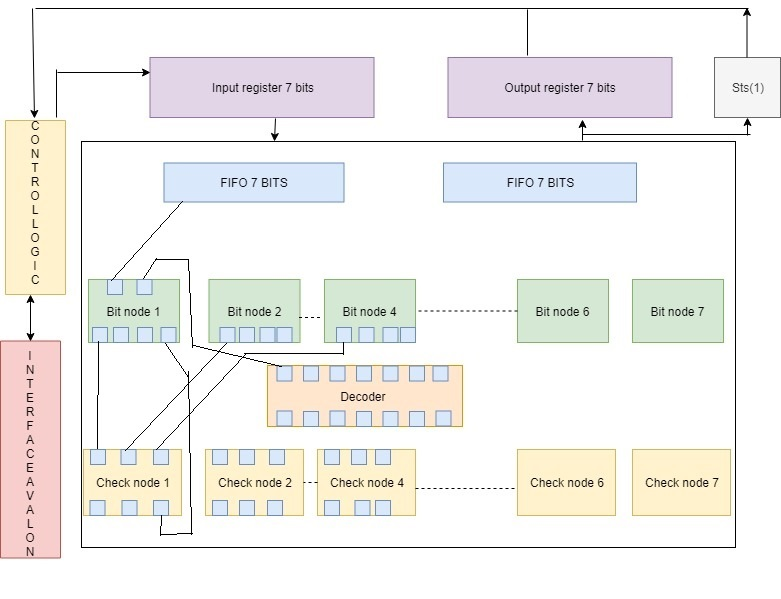
\includegraphics[width=\linewidth]{LDPC-Block.jpg}
\label{fig:bd}
\end{figure}

Appendix A describes in detail how the RTL design of the LDPC core and its
components were carried out. The design is hierarchical:

\begin{figure}[hbt]
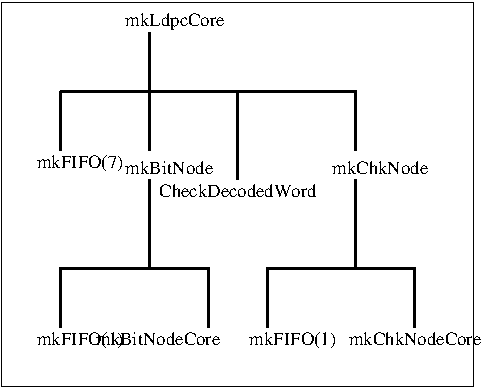
\includegraphics{des-hier.pdf}
\label{fig:dh}
\end{figure}

\section{From RTL to GDSII}
In the course of the project we experimented with two different design flows
to realise a circuit for the LDPC decoder. The starting point of both flows
was after the design had been sufficiently verified through functional
simulations as well as by running as an Avalon slave on the DE-Nano board.

\subsection{Bottom-up Flow Using Java Electric}

Figure~\ref{fig:flow1} captures the steps involved in a bottom-up flow using
the Electric tool-flow introduced as part of the course:

\begin{figure}[hbt]
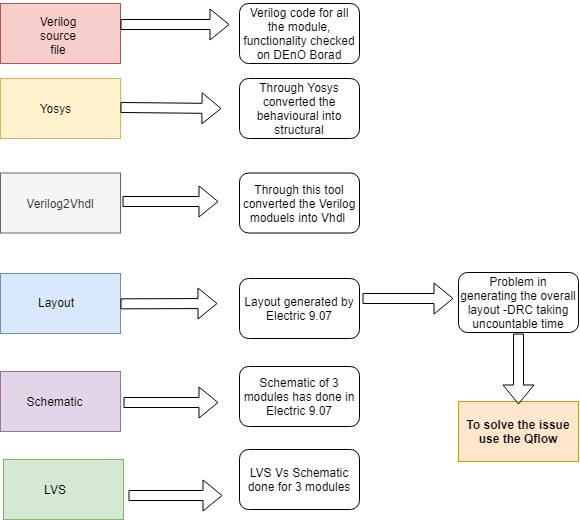
\includegraphics[width=\linewidth]{FLOW1.jpg}
\label{fig:flow}
\caption{Flow using Java Electric}
\end{figure}

The Yosys synthesis tool reads in behavioural RTL and generates a structural
netlist, given a cell library. The tool uses the abc tool in the background to
actually do the synthesis. 

The structural RTL is then converted to structural VHDL. This step usually
involved running multiple scripts to get it into just the correct format for
input to the Electric tool suite.

In the bottom-up flow we begin at the lowest level of the hierarchy,
individually, synthesizing, and then creating layouts and schematic for each
module. Each individual module is taken through DRC and LVS.

As the leaf module got bigger, manual schematic entry became problemmatic. So
we decided to carry out LVS by comparing the spice netlist dumped from the
layout versus the spice netlist created by Yosys. 

Java Electric was not able to check DRC on the complete design repeatedly
crashing after a few hours of running DRC. 

\subsubsection{Manual stitching in Electric}
We have used electric 9.07 using bottom-up appraoch for creating layout out of
the VHDL files. It has created layout for each node with successful design
rule check(DRC) and earlier the plan was to make layout for individual module
and then make layout manually for the overall LDPC decoder using these
individual module. But the layouts for the individual modules were quite big
and creating layout for the whole circuit using those big layout became
extremely difficult. We are using 7 bitnodes and 7 checknodes and for
each node there is an individual layout means 14 layouts only for these
bitnodes and checknodes, leaving other nodes aside. This was becoming
something which was going out of reach for the mannual layout.

Then we decided to combine all the vhdl code files for respective modules in
the vhdl code file of the top level circuit and tried to generate the
automatic layout from electric 9.07. We have tried to make changes in the
placement settings,routing settings and to use metal layers more than 2 but
electric remains unresponsive and creating layout with the default settings.
But there was a problem in running DRC for this top level circuit layout
because it was taking too long to complete the DRC and still not displaying
the results/errors.To solve this problem we decided to shift towards Qflow
open circuit design tool.

\subsection{Top-down Flow Using Q-Flow}
The limitations with DRC on Java Electric led us to explore an alternate
design flow. For this we settled on a top-down flow called qflow, which
integrates a set of open-source tools. In this flow we have to explicitly do
placement and routing - it is not integrated under a single tool like Java
Electric. On the other hand, this flow has complete PDKs for 350nm and 180nm
processes which makes it possible to generate a GDS-II.

\begin{figure}[hbt]
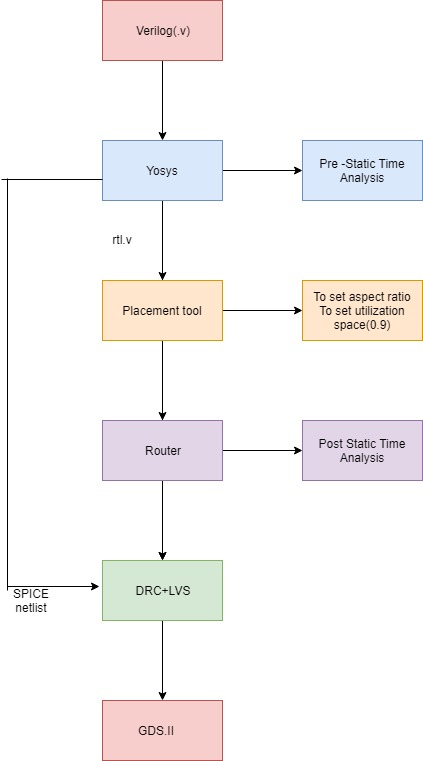
\includegraphics[scale=0.5]{FLOW2.jpg}
\label{fig:flow-q}
\caption{Flow using QFlow}
\end{figure}

The other big difference from the Electric based flow is the use of a top-down
approach where the whole LDPC core is flattened allowing the place and route
tool greater flexibility. We also did try a bottom-up approach with this flow,
but it resulted in several DRC violations at the top-level which we haven't
yet managed to debug.

The QFlow based flow also integrates static timing analysis -- something which
was missing on the Electric based flow. 

\section{Results}
These results were obtained using OSU's 350nm PDK. A hierarchical layout and
flat layout are contrasted on figure~\ref{fig:routes}. The flat layout is
clearly superior in terms of timing and area due to the much higher compaction
obtained by automatic layout.

\begin{figure}[!ht]
   \subfloat[Hierarchical \label{route:h}]{
      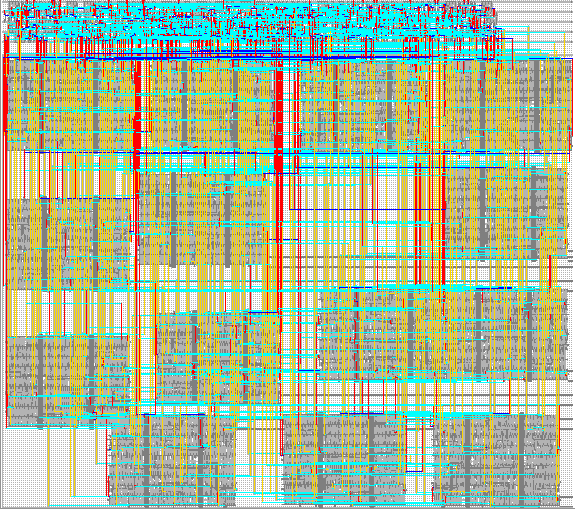
\includegraphics[width=0.45\linewidth]{routing.png}
   }
   \subfloat[Flat \label{route:f}]{
      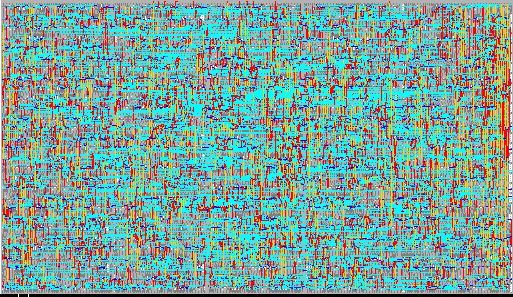
\includegraphics[width=0.45\linewidth]{routing-flat.png}
   }
   \caption{Routes -- Hierarchical and Flat}
\end{figure}

From our bottom-up synthesis of the bitnode and checknode, the pre and
post-layout maximum operating frequencies are:

\begin{description}
   \item[mkBitNode:] 535.41 MHz, 533 MHz
   \item[mkChkNode:] 481.60 MHz, 479.11 MHz
\end{description}

\appendix
\include{LdpcTop}
% vim: set tabstop=8:softtabstop=4:shiftwidth=4:textwidth:78:formatoptions+=t% ===> this file was generated automatically by noweave --- better not edit it
\section{Nodes of the LDPC Decoder}
The work-horses of the decoder are the bit and check nodes. These iteratively
decode the input code-word passing the partially decoded result back-and-forth
for a fixed number of iterations.

\nwfilename{Nodes.bsv.nw}\nwbegincode{1}\sublabel{NW1v8dKs-To6Q8-1}\nwmargintag{{\nwtagstyle{}\subpageref{NW1v8dKs-To6Q8-1}}}\moddef{boilerplate~{\nwtagstyle{}\subpageref{NW1v8dKs-To6Q8-1}}}\endmoddef\nwstartdeflinemarkup\nwenddeflinemarkup
// EE-705 Course Project -- LDPC Decoder

package Nodes;

// -----------------------------------------------------------------
// This package defines:
//
//    ChkNode        : Interface to the Check Nodes
//    BitNode        : Interface to the Bit Nodes
//    mkChkNode      : Micro-arch of the Check Node
//    mkBitNode      : Micro-arch of the Bit Node
//    mkBitNodeCore  : Core computation of the Bit Node
//    mkChkNodeCore  : Core computation of the Check Node
//
//    v1.0           : The nodes can handle one code-word at a time
//
// -----------------------------------------------------------------

import ClientServer     :: *;
import GetPut           :: *;
import FIFO             :: *;
import Vector           :: *;
import LdpcTypes        :: *;

\LA{}type definitions~{\nwtagstyle{}\subpageref{NW1v8dKs-4O0RoX-1}}\RA{}

\LA{}module definition~{\nwtagstyle{}\subpageref{NW1v8dKs-1nQrPK-1}}\RA{}

\nwnotused{boilerplate}\nwendcode{}\nwbegindocs{2}\nwdocspar
The Bit-node and the Check-node are the two types of computation nodes in
the LDPC decoder. One iteration consists of processing at both of these
nodes. The interconnections between them is described by the incidence
matrix (H matrix).

\nwenddocs{}\nwbegincode{3}\sublabel{NW1v8dKs-4O0RoX-1}\nwmargintag{{\nwtagstyle{}\subpageref{NW1v8dKs-4O0RoX-1}}}\moddef{type definitions~{\nwtagstyle{}\subpageref{NW1v8dKs-4O0RoX-1}}}\endmoddef\nwstartdeflinemarkup\nwusesondefline{\\{NW1v8dKs-To6Q8-1}}\nwenddeflinemarkup
\LA{}interface definition~{\nwtagstyle{}\subpageref{NW1v8dKs-3l1BOL-1}}\RA{}

\nwused{\\{NW1v8dKs-To6Q8-1}}\nwendcode{}\nwbegindocs{4}\nwdocspar
\section{Interfaces of the Bit and Check Nodes}
Two interface types, one each for the Bit and Check nodes are defined in
this package. Both interfaces are parameterized by the numeric types
{\Tt{}NConnections\nwendquote}.

The numeric type, {\Tt{}NConnections\nwendquote} indicates the number of ones along a
particular row of the incidence matrix, which is also same as the number of
ones along a particular column of the incidence matrix.

\nwenddocs{}\nwbegincode{5}\sublabel{NW1v8dKs-3l1BOL-1}\nwmargintag{{\nwtagstyle{}\subpageref{NW1v8dKs-3l1BOL-1}}}\moddef{interface definition~{\nwtagstyle{}\subpageref{NW1v8dKs-3l1BOL-1}}}\endmoddef\nwstartdeflinemarkup\nwusesondefline{\\{NW1v8dKs-4O0RoX-1}}\nwprevnextdefs{\relax}{NW1v8dKs-3l1BOL-2}\nwenddeflinemarkup
// NConnections indicates the number of connections that a particular
// check-node has with the bit-nodes
interface ChkNode;
   interface Vector #(NConnections, Put #(Symbol)) b2c;
   interface Vector #(NConnections, Get #(Symbol)) c2b;
endinterface

\nwalsodefined{\\{NW1v8dKs-3l1BOL-2}\\{NW1v8dKs-3l1BOL-3}}\nwused{\\{NW1v8dKs-4O0RoX-1}}\nwendcode{}\nwbegindocs{6}\nwdocspar
A check node can be imagined to receive {\Tt{}Symbol\nwendquote} values from a vector
of interfaces. Each interface is connected to a different bit nodes. In
turn, the check node returns a single {\Tt{}Symbol\nwendquote} values broadcast to all
its bit nodes.

\nwenddocs{}\nwbegincode{7}\sublabel{NW1v8dKs-3l1BOL-2}\nwmargintag{{\nwtagstyle{}\subpageref{NW1v8dKs-3l1BOL-2}}}\moddef{interface definition~{\nwtagstyle{}\subpageref{NW1v8dKs-3l1BOL-1}}}\plusendmoddef\nwstartdeflinemarkup\nwusesondefline{\\{NW1v8dKs-4O0RoX-1}}\nwprevnextdefs{NW1v8dKs-3l1BOL-1}{NW1v8dKs-3l1BOL-3}\nwenddeflinemarkup
// NConnections indicates the number of connections that a particular
// bit-node has with the check-nodes
interface BitNode;
   // Bit Node-Check Node Interface
   interface Vector #(NConnections, Put #(Symbol)) c2b;
   interface Get #(Symbol) b2c;

\nwused{\\{NW1v8dKs-4O0RoX-1}}\nwendcode{}\nwbegindocs{8}\nwdocspar
The inverse applies for the bit-check node connection from the bit
node's perspective. It sends a single {\Tt{}Symbol\nwendquote} values broadcast to all
its check nodes, and collects responses through a vector of interfaces,
each connected to a different check node.
 
\nwenddocs{}\nwbegincode{9}\sublabel{NW1v8dKs-3l1BOL-3}\nwmargintag{{\nwtagstyle{}\subpageref{NW1v8dKs-3l1BOL-3}}}\moddef{interface definition~{\nwtagstyle{}\subpageref{NW1v8dKs-3l1BOL-1}}}\plusendmoddef\nwstartdeflinemarkup\nwusesondefline{\\{NW1v8dKs-4O0RoX-1}}\nwprevnextdefs{NW1v8dKs-3l1BOL-2}{\relax}\nwenddeflinemarkup

   // External interfaces for receving code word and returning result
   interface Put     #(Symbol)   codeIn;
   interface Get     #(Symbol)   dataOut;

endinterface

// -----------------------------------------------------------------

\nwused{\\{NW1v8dKs-4O0RoX-1}}\nwendcode{}\nwbegindocs{10}\nwdocspar
In addition to the sub-interfaces to connect the check
and bit nodes, bit nodes also have the additional interfaces to receive the
code and send back the decoded data. Since each bit-node only deals with a
part of the code-word, it is sufficient to receive those symbols only. The
final decoded word is also constructed from the responses of the different
bit-nodes. Each bit node receives one symbol to decode at a time.

\nwenddocs{}\nwbegindocs{11}\nwdocspar
\section{The Bit Node}
The {\Tt{}mkBitNode\nwendquote} module receives the code word and initiates an
iterations  Based on {\Tt{}NConnections\nwendquote} it is connected to a set of
{\Tt{}mkChkNodes\nwendquote} representing the edges of the bipartite tanner graph. The
{\Tt{}mkBitNode\nwendquote} provides an interface of type {\Tt{}BitNode\nwendquote}.

\nwenddocs{}\nwbegincode{12}\sublabel{NW1v8dKs-1nQrPK-1}\nwmargintag{{\nwtagstyle{}\subpageref{NW1v8dKs-1nQrPK-1}}}\moddef{module definition~{\nwtagstyle{}\subpageref{NW1v8dKs-1nQrPK-1}}}\endmoddef\nwstartdeflinemarkup\nwusesondefline{\\{NW1v8dKs-To6Q8-1}}\nwprevnextdefs{\relax}{NW1v8dKs-1nQrPK-2}\nwenddeflinemarkup
// Core function of the bitNode
\LA{}functions bitNode~{\nwtagstyle{}\subpageref{NW1v8dKs-2TR1lR-1}}\RA{}

//
// Bit Node Module definition
(* synthesize *)
module mkBitNode (BitNode);
   \LA{}state bitNode~{\nwtagstyle{}\subpageref{NW1v8dKs-3Q7ADd-1}}\RA{}
   \LA{}rules bitNode~{\nwtagstyle{}\subpageref{NW1v8dKs-2ke5KA-1}}\RA{}
   \LA{}interfaces bitNode~{\nwtagstyle{}\subpageref{NW1v8dKs-469JCS-1}}\RA{}
\LA{}wrap up bitNode~{\nwtagstyle{}\subpageref{NW1v8dKs-oZLgz-1}}\RA{}
// -----------------------------------------------------------------

\nwalsodefined{\\{NW1v8dKs-1nQrPK-2}}\nwused{\\{NW1v8dKs-To6Q8-1}}\nwendcode{}\nwbegindocs{13}\nwdocspar
The input FIFO {\Tt{}ffCodeIn\nwendquote} receives the symbol of the code word meant for this
bit-node. The output FIFO {\Tt{}ffDataOut\nwendquote} holds the decoded symbol.

\nwenddocs{}\nwbegincode{14}\sublabel{NW1v8dKs-3Q7ADd-1}\nwmargintag{{\nwtagstyle{}\subpageref{NW1v8dKs-3Q7ADd-1}}}\moddef{state bitNode~{\nwtagstyle{}\subpageref{NW1v8dKs-3Q7ADd-1}}}\endmoddef\nwstartdeflinemarkup\nwusesondefline{\\{NW1v8dKs-1nQrPK-1}}\nwprevnextdefs{\relax}{NW1v8dKs-3Q7ADd-2}\nwenddeflinemarkup
// Sub-modules and state
// Input FIFO - code word
FIFO  #(Symbol)   ffCodeIn    <- mkFIFO;

// Output FIFO - decoded code word
FIFO  #(Symbol)   ffDataOut   <- mkFIFO;

\nwalsodefined{\\{NW1v8dKs-3Q7ADd-2}}\nwused{\\{NW1v8dKs-1nQrPK-1}}\nwendcode{}\nwbegindocs{15}\nwdocspar
The {\Tt{}ffB2C\nwendquote} FIFO holds the partially processed codeword. The contents of
this FIFO will be consumed by the check node when they are ready. The
{\Tt{}vffC2B\nwendquote} FIFO receives partially processed codewords from the check nodes
and this completes one iteration of processing.

\nwenddocs{}\nwbegincode{16}\sublabel{NW1v8dKs-3Q7ADd-2}\nwmargintag{{\nwtagstyle{}\subpageref{NW1v8dKs-3Q7ADd-2}}}\moddef{state bitNode~{\nwtagstyle{}\subpageref{NW1v8dKs-3Q7ADd-1}}}\plusendmoddef\nwstartdeflinemarkup\nwusesondefline{\\{NW1v8dKs-1nQrPK-1}}\nwprevnextdefs{NW1v8dKs-3Q7ADd-1}{\relax}\nwenddeflinemarkup
// Partially processed codeword meant for the checknodes
FIFO  #(Symbol)      ffB2C       <- mkFIFO;

// Partially processed codeword from the checknodes
Vector #(
     NConnections
   , FIFO #(Symbol)) vffC2B      <- replicateM (mkFIFO);

\nwused{\\{NW1v8dKs-1nQrPK-1}}\nwendcode{}\nwbegindocs{17}\nwdocspar
Behaviour is described in terms of atomic sets of actions called rules.
The rule, {\Tt{}rlProcessFirstIteration\nwendquote} executes the actions for the first
iteration of processing a new code word. 

\begin{itemize}
\item Consume the codeword which is currently in {\Tt{}ffCodeIn\nwendquote}
\item Carry out some initial processing on the codeword
\item Enqueue the result into the {\Tt{}ffB2C\nwendquote} for checknode processing
\item Update the iteration count - this is updated by $2$ as the count is
maintained only in the bit node, and the check node acts as a purely
passive device.
\end{itemize}

The first iteration is counted when the code word goes through the check
node for the first time.

\nwenddocs{}\nwbegincode{18}\sublabel{NW1v8dKs-2ke5KA-1}\nwmargintag{{\nwtagstyle{}\subpageref{NW1v8dKs-2ke5KA-1}}}\moddef{rules bitNode~{\nwtagstyle{}\subpageref{NW1v8dKs-2ke5KA-1}}}\endmoddef\nwstartdeflinemarkup\nwusesondefline{\\{NW1v8dKs-1nQrPK-1}}\nwprevnextdefs{\relax}{NW1v8dKs-2ke5KA-2}\nwenddeflinemarkup
// Rules and behaviour

// Rule to process new data received from the top-level
rule rlProcessNewData;
   // As this is the first iteration, consume the codeword which is
   // currently in ffCodeIn. Carry out the computation on the codeword
   let codeIn = ffCodeIn.first; ffCodeIn.deq;

   // Send the output to the check nodes
   ffB2C.enq (codeIn);
endrule

// -----------------------------------------------------------------

\nwalsodefined{\\{NW1v8dKs-2ke5KA-2}}\nwused{\\{NW1v8dKs-1nQrPK-1}}\nwendcode{}\nwbegindocs{19}\nwdocspar
The function {\Tt{}fnBitNodeCore\nwendquote}, carries out the actual bit
manipulation of the codeword symbols as per the min-sum-algorithm. The
noinline attribute ensures that a separate verilog module is generated for the
function. In fact this module was developed entirely in verilog, and then
merged with this module later.

\nwenddocs{}\nwbegincode{20}\sublabel{NW1v8dKs-2TR1lR-1}\nwmargintag{{\nwtagstyle{}\subpageref{NW1v8dKs-2TR1lR-1}}}\moddef{functions bitNode~{\nwtagstyle{}\subpageref{NW1v8dKs-2TR1lR-1}}}\endmoddef\nwstartdeflinemarkup\nwusesondefline{\\{NW1v8dKs-1nQrPK-1}}\nwenddeflinemarkup
(* noinline *)
function Symbol fnBitNodeCore (Vector #(NConnections, Symbol) i);
   return ((i[1]&i[2])|(i[0]&i[2])|(i[0]&i[1]));
endfunction

\nwused{\\{NW1v8dKs-1nQrPK-1}}\nwendcode{}\nwbegindocs{21}\nwdocspar
The rule {\Tt{}rlProcessChkNodeResult\nwendquote} executes the actions on receiving a
response from the check node. The input for these iterations is
from the partially processed word in {\Tt{}vffC2B\nwendquote}.

\begin{itemize}
\item Consume the codeword which is currently in {\Tt{}vffC2B\nwendquote}
\item Carry out the computation on the codeword as per
{\Tt{}fnBitNodeCore\nwendquote}
\item Enqueue the result into the {\Tt{}ffDataOut\nwendquote} for global checks at the
top-level
\end{itemize}

\nwenddocs{}\nwbegincode{22}\sublabel{NW1v8dKs-2ke5KA-2}\nwmargintag{{\nwtagstyle{}\subpageref{NW1v8dKs-2ke5KA-2}}}\moddef{rules bitNode~{\nwtagstyle{}\subpageref{NW1v8dKs-2ke5KA-1}}}\plusendmoddef\nwstartdeflinemarkup\nwusesondefline{\\{NW1v8dKs-1nQrPK-1}}\nwprevnextdefs{NW1v8dKs-2ke5KA-1}{\relax}\nwenddeflinemarkup
\LA{}mutex pragma~{\nwtagstyle{}\subpageref{NW1v8dKs-4c5Jhr-1}}\RA{}
// Rule to process remaining iterations
rule rlProcessChkNodeResult;
   // As this iteration works of a partial result from the checknode,
   // the input comes from the vector of fifos vffC2B
   Vector #(NConnections, Symbol) codeIn;
   for (Integer i=0; i<valueOf(NConnections); i=i+1) begin
      codeIn[i] = vffC2B[i].first;
      vffC2B[i].deq;
   end

   // Send the processed code word to the output
   ffDataOut.enq (fnBitNodeCore (codeIn));
endrule

// -----------------------------------------------------------------

\nwused{\\{NW1v8dKs-1nQrPK-1}}\nwendcode{}\nwbegindocs{23}\nwdocspar
The {\Tt{}rlProcessChkNodeResult\nwendquote} rule will only run when there is a
partial result from the check nodes. On the other hand the
{\Tt{}rlProcessNewData\nwendquote} will only run when there is new data input from the
top-level. These two rules are mutually exclusive in a non-pipelined
implementation such as this one. The mutex pragma specifies this as an
assertion to the compiler.

\nwenddocs{}\nwbegincode{24}\sublabel{NW1v8dKs-4c5Jhr-1}\nwmargintag{{\nwtagstyle{}\subpageref{NW1v8dKs-4c5Jhr-1}}}\moddef{mutex pragma~{\nwtagstyle{}\subpageref{NW1v8dKs-4c5Jhr-1}}}\endmoddef\nwstartdeflinemarkup\nwusesondefline{\\{NW1v8dKs-2ke5KA-2}}\nwenddeflinemarkup
(* mutually_exclusive = "rlProcessChkNodeResult, rlProcessNewData" *)

\nwused{\\{NW1v8dKs-2ke5KA-2}}\nwendcode{}\nwbegindocs{25}\nwdocspar
Creating the interfaces simply involves stitching up the connections to the
input and output FIFOs using library functions -- {\Tt{}toPut\nwendquote}, {\Tt{}toGet\nwendquote}.
Since the {\Tt{}c2b\nwendquote} interface is a vector, the {\Tt{}map\nwendquote} higher-order function is
applied.

\nwenddocs{}\nwbegincode{26}\sublabel{NW1v8dKs-469JCS-1}\nwmargintag{{\nwtagstyle{}\subpageref{NW1v8dKs-469JCS-1}}}\moddef{interfaces bitNode~{\nwtagstyle{}\subpageref{NW1v8dKs-469JCS-1}}}\endmoddef\nwstartdeflinemarkup\nwusesondefline{\\{NW1v8dKs-1nQrPK-1}}\nwenddeflinemarkup
// Interface
interface codeIn     = toPut (ffCodeIn);
interface dataOut    = toGet (ffDataOut);
interface c2b        = map (toPut, vffC2B);
interface b2c        = toGet (ffB2C);

// -----------------------------------------------------------------

\nwused{\\{NW1v8dKs-1nQrPK-1}}\nwendcode{}\nwbegincode{27}\sublabel{NW1v8dKs-oZLgz-1}\nwmargintag{{\nwtagstyle{}\subpageref{NW1v8dKs-oZLgz-1}}}\moddef{wrap up bitNode~{\nwtagstyle{}\subpageref{NW1v8dKs-oZLgz-1}}}\endmoddef\nwstartdeflinemarkup\nwusesondefline{\\{NW1v8dKs-1nQrPK-1}}\nwenddeflinemarkup
endmodule : mkBitNode

\nwused{\\{NW1v8dKs-1nQrPK-1}}\nwendcode{}\nwbegindocs{28}\nwdocspar
\section{The Check Node}
The {\Tt{}mkChkNode\nwendquote} module receives the partially decoded code word from
the {\Tt{}mkBitNode\nwendquote}. It operates in \emph{slave} mode and processes all
inputs in the same manner. The {\Tt{}mkChkNode\nwendquote} does not keep track of
iterations. The {\Tt{}mkChkNode\nwendquote} provides an interface of type {\Tt{}ChkNode\nwendquote}.

\nwenddocs{}\nwbegincode{29}\sublabel{NW1v8dKs-1nQrPK-2}\nwmargintag{{\nwtagstyle{}\subpageref{NW1v8dKs-1nQrPK-2}}}\moddef{module definition~{\nwtagstyle{}\subpageref{NW1v8dKs-1nQrPK-1}}}\plusendmoddef\nwstartdeflinemarkup\nwusesondefline{\\{NW1v8dKs-To6Q8-1}}\nwprevnextdefs{NW1v8dKs-1nQrPK-1}{\relax}\nwenddeflinemarkup
// Core function of the check-node
\LA{}functions checkNode~{\nwtagstyle{}\subpageref{NW1v8dKs-oud5A-1}}\RA{}

//
// Check Node Module definition
(* synthesize *)
module mkChkNode (ChkNode);
   \LA{}state checkNode~{\nwtagstyle{}\subpageref{NW1v8dKs-2jCWTO-1}}\RA{}
   \LA{}rules checkNode~{\nwtagstyle{}\subpageref{NW1v8dKs-4bVYKS-1}}\RA{}
   \LA{}interfaces checkNode~{\nwtagstyle{}\subpageref{NW1v8dKs-1mJizB-1}}\RA{}
   \LA{}wrap up checkNode~{\nwtagstyle{}\subpageref{NW1v8dKs-HAQpJ-1}}\RA{}
// -----------------------------------------------------------------

\nwused{\\{NW1v8dKs-To6Q8-1}}\nwendcode{}\nwbegindocs{30}\nwdocspar
The input FIFOs {\Tt{}vffB2C\nwendquote} receives the partially processed part of the code
word meant for this check-node. The output FIFO {\Tt{}ffC2B\nwendquote} holds the
partially decoded code word.

\nwenddocs{}\nwbegincode{31}\sublabel{NW1v8dKs-2jCWTO-1}\nwmargintag{{\nwtagstyle{}\subpageref{NW1v8dKs-2jCWTO-1}}}\moddef{state checkNode~{\nwtagstyle{}\subpageref{NW1v8dKs-2jCWTO-1}}}\endmoddef\nwstartdeflinemarkup\nwusesondefline{\\{NW1v8dKs-1nQrPK-2}}\nwenddeflinemarkup
// Sub-modules and state
// Input FIFO - code word
Vector #(
     NConnections
   , FIFO #(Symbol)) vffB2C        <- replicateM (mkFIFO);

// Output FIFO - decoded code word
Vector #(
     NConnections
   , FIFO #(Symbol)) vffC2B        <- replicateM (mkFIFO);

\nwused{\\{NW1v8dKs-1nQrPK-2}}\nwendcode{}\nwbegindocs{32}\nwdocspar
The rule {\Tt{}rlProcessIteration\nwendquote} executes the actions for process the
input from the bit nodes.

\begin{itemize}
\item Consume the codeword which is currently in {\Tt{}vffB2C\nwendquote}
\item Carry out the computation on the codeword
\item Enqueue the result into the {\Tt{}ffC2B\nwendquote} for bit-node processing
\end{itemize}

\nwenddocs{}\nwbegincode{33}\sublabel{NW1v8dKs-4bVYKS-1}\nwmargintag{{\nwtagstyle{}\subpageref{NW1v8dKs-4bVYKS-1}}}\moddef{rules checkNode~{\nwtagstyle{}\subpageref{NW1v8dKs-4bVYKS-1}}}\endmoddef\nwstartdeflinemarkup\nwusesondefline{\\{NW1v8dKs-1nQrPK-2}}\nwenddeflinemarkup
// Rules and behaviour
rule rlProcessIteration;
   // get the partial result
   Vector #(NConnections, Symbol) codeIn;
   for (Integer i=0; i<valueOf(NConnections); i=i+1) begin
      codeIn[i] = vffB2C[i].first;
      vffB2C[i].deq;
   end

   // Send the partial result to the bit node
   let res = fnChkNodeCore (codeIn);
   for (Integer i=0; i<valueOf(NConnections); i=i+1)
      vffC2B[i].enq (res[i]);
endrule

// -----------------------------------------------------------------

\nwused{\\{NW1v8dKs-1nQrPK-2}}\nwendcode{}\nwbegindocs{34}\nwdocspar
The function {\Tt{}fnChkNodeCore\nwendquote}, carries out the actual bit
manipulation of the codeword bits as per the min-sum algorithm. The
noinline attribute ensures that a separate verilog module is generated for the
function.

\nwenddocs{}\nwbegincode{35}\sublabel{NW1v8dKs-oud5A-1}\nwmargintag{{\nwtagstyle{}\subpageref{NW1v8dKs-oud5A-1}}}\moddef{functions checkNode~{\nwtagstyle{}\subpageref{NW1v8dKs-oud5A-1}}}\endmoddef\nwstartdeflinemarkup\nwusesondefline{\\{NW1v8dKs-1nQrPK-2}}\nwenddeflinemarkup
(* noinline *)
function Vector#(NConnections, Symbol) fnChkNodeCore (Vector #(NConnections, Symbol) i);
   Vector #(NConnections, Symbol) o = newVector;
   o[0]=i[1]^i[2];
   o[1]=i[0]^i[2];
   o[2]=i[0]^i[1];
   return (o);
endfunction

\nwused{\\{NW1v8dKs-1nQrPK-2}}\nwendcode{}\nwbegindocs{36}\nwdocspar
Creating the interfaces simply involves stitching up the connections to the
input and output FIFOs using library functions -- {\Tt{}toPut\nwendquote} and {\Tt{}toGet\nwendquote}.
Since the {\Tt{}b2c\nwendquote} interface is a vector, the {\Tt{}map\nwendquote} higher-order function is
applied.

\nwenddocs{}\nwbegincode{37}\sublabel{NW1v8dKs-1mJizB-1}\nwmargintag{{\nwtagstyle{}\subpageref{NW1v8dKs-1mJizB-1}}}\moddef{interfaces checkNode~{\nwtagstyle{}\subpageref{NW1v8dKs-1mJizB-1}}}\endmoddef\nwstartdeflinemarkup\nwusesondefline{\\{NW1v8dKs-1nQrPK-2}}\nwenddeflinemarkup
// Interface
interface c2b = map (toGet, vffC2B);
interface b2c = map (toPut, vffB2C);

// -----------------------------------------------------------------

\nwused{\\{NW1v8dKs-1nQrPK-2}}\nwendcode{}

\nwixlogsorted{c}{{boilerplate}{NW1v8dKs-To6Q8-1}{\nwixd{NW1v8dKs-To6Q8-1}}}%
\nwixlogsorted{c}{{functions bitNode}{NW1v8dKs-2TR1lR-1}{\nwixu{NW1v8dKs-1nQrPK-1}\nwixd{NW1v8dKs-2TR1lR-1}}}%
\nwixlogsorted{c}{{functions checkNode}{NW1v8dKs-oud5A-1}{\nwixu{NW1v8dKs-1nQrPK-2}\nwixd{NW1v8dKs-oud5A-1}}}%
\nwixlogsorted{c}{{interface definition}{NW1v8dKs-3l1BOL-1}{\nwixu{NW1v8dKs-4O0RoX-1}\nwixd{NW1v8dKs-3l1BOL-1}\nwixd{NW1v8dKs-3l1BOL-2}\nwixd{NW1v8dKs-3l1BOL-3}}}%
\nwixlogsorted{c}{{interfaces bitNode}{NW1v8dKs-469JCS-1}{\nwixu{NW1v8dKs-1nQrPK-1}\nwixd{NW1v8dKs-469JCS-1}}}%
\nwixlogsorted{c}{{interfaces checkNode}{NW1v8dKs-1mJizB-1}{\nwixu{NW1v8dKs-1nQrPK-2}\nwixd{NW1v8dKs-1mJizB-1}}}%
\nwixlogsorted{c}{{module definition}{NW1v8dKs-1nQrPK-1}{\nwixu{NW1v8dKs-To6Q8-1}\nwixd{NW1v8dKs-1nQrPK-1}\nwixd{NW1v8dKs-1nQrPK-2}}}%
\nwixlogsorted{c}{{mutex pragma}{NW1v8dKs-4c5Jhr-1}{\nwixu{NW1v8dKs-2ke5KA-2}\nwixd{NW1v8dKs-4c5Jhr-1}}}%
\nwixlogsorted{c}{{rules bitNode}{NW1v8dKs-2ke5KA-1}{\nwixu{NW1v8dKs-1nQrPK-1}\nwixd{NW1v8dKs-2ke5KA-1}\nwixd{NW1v8dKs-2ke5KA-2}}}%
\nwixlogsorted{c}{{rules checkNode}{NW1v8dKs-4bVYKS-1}{\nwixu{NW1v8dKs-1nQrPK-2}\nwixd{NW1v8dKs-4bVYKS-1}}}%
\nwixlogsorted{c}{{state bitNode}{NW1v8dKs-3Q7ADd-1}{\nwixu{NW1v8dKs-1nQrPK-1}\nwixd{NW1v8dKs-3Q7ADd-1}\nwixd{NW1v8dKs-3Q7ADd-2}}}%
\nwixlogsorted{c}{{state checkNode}{NW1v8dKs-2jCWTO-1}{\nwixu{NW1v8dKs-1nQrPK-2}\nwixd{NW1v8dKs-2jCWTO-1}}}%
\nwixlogsorted{c}{{type definitions}{NW1v8dKs-4O0RoX-1}{\nwixu{NW1v8dKs-To6Q8-1}\nwixd{NW1v8dKs-4O0RoX-1}}}%
\nwixlogsorted{c}{{wrap up bitNode}{NW1v8dKs-oZLgz-1}{\nwixu{NW1v8dKs-1nQrPK-1}\nwixd{NW1v8dKs-oZLgz-1}}}%
\nwixlogsorted{c}{{wrap up checkNode}{NW1v8dKs-HAQpJ-1}{\nwixu{NW1v8dKs-1nQrPK-2}\nwixd{NW1v8dKs-HAQpJ-1}}}%
\nwbegincode{38}\sublabel{NW1v8dKs-HAQpJ-1}\nwmargintag{{\nwtagstyle{}\subpageref{NW1v8dKs-HAQpJ-1}}}\moddef{wrap up checkNode~{\nwtagstyle{}\subpageref{NW1v8dKs-HAQpJ-1}}}\endmoddef\nwstartdeflinemarkup\nwusesondefline{\\{NW1v8dKs-1nQrPK-2}}\nwenddeflinemarkup
endmodule : mkChkNode
endpackage
\nwused{\\{NW1v8dKs-1nQrPK-2}}\nwendcode{}

\end{document}
